\chapter{Rumore termico}

\begin{figure}[h]
    \centering
    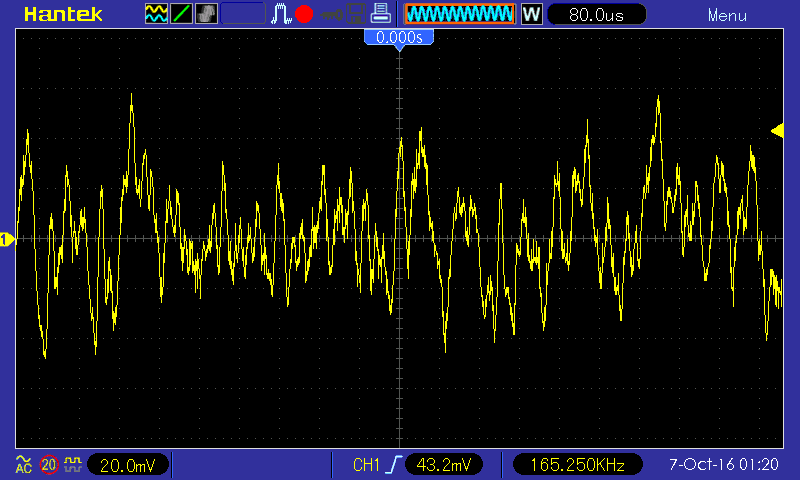
\includegraphics[scale = 0.7]{whiteNoise.png} 
\end{figure}  

\newpage

\section{Un esempio di processo stocastico: il rumore termico}

Un esempio molto importante di processo stocastico è costituito dal rumore termico. \newline 

Il rumore termico è dovuto all'agitazione termica degli elettroni liberi degli elettroni liberi nei conduttori. \newline 

Gli elettroni, infatti, trovandosi ad una temperatura diversa dallo zero assoluto 
($T = 0^{\circ} K$ è l'unica condizione che consetirebbe di annullare il rumore termico) 
si muovono con moto caotico e disordinato producendo ai capi del conduttore una differenza di potenziale osservabile. \newline 

D'altro canto un rumore con caratteristiche analoghe a quelle del rumore termico è anche presente 
nelle reti attive, contententi generatori controllati o indipendenti, ove esso è dovuto, oltre che 
all'agitazione termcica, anche alle fluttuazioni di corrnte o di tensione dei generatori. \newline 


Si può affermare che si tratta di un processo stazionario ed ergodico, per cui la descrizione statistica del primo ordine 
è fattibile sulla base dell'osservazione del processo in un generico istante. \newline 

Per il fatto che la tensione di rumore è il risultato della somma di numerosissimi contributi, nessuno dei quali è dominante 
e che possono essere assunti, con buona approssimazione, tra loro indipendenti, è lecito applicare il teorema-limite centrale. \newline 

Considerando per una tensione v, per qualunque t, è una variabile gaussiana con valor medio nulla e varianza $\sigma_v ^{2}$. \newline 

Si ha dunque: 

{
    \Large 
    \begin{equation}
        f(v) = \frac{1}{\sqrt{2 \pi} \sigma_v } \exp(- \frac{v^{2}}{2 \sigma_v ^{2}})
    \end{equation}
}

Per completare la descrizione statistica, è necessario esplicitare il valore della varianza. \newline 

Essendo il valore medio uguale a zero, la varianza di v coincide con il valore quadratico medio; si ha cioè: 

{
    \Large 
    \begin{equation}
        \sigma_v ^{2} = <v^{2}> - <v>^{2} = <v^{2}>
    \end{equation}
}

Essendo il processo ergodico, il valore ergodico, il valore quadratico medio coincide con la potenza del processo. \newline 

In definitiva, la varianza della variabile aleatoria v può essere estratta da una valutazione di potenza. \newline 

La potenza del segnale di rumore v(t) può essere misurata e si scopre che essa cresce proporzionalmente con: 

\begin{itemize}
    \item il valore della resistenza R 
    \item il valore della temperatura assoluta T a cui si trova la resistenza 
    \item il valore della banda passante B del filtro interno all'apparato con cui si effettua la misura 
\end{itemize} 

La costante di proporzionalità è pari a 4K, dove: 

{
    \Large 
    \begin{equation}
        K = 1.38 \cdot 10^{-23} \frac{J}{^{\circ} K}
    \end{equation}
}

è la costante di Boltzmann. \newline 

In definitiva si ha dunque: 

{
    \Large 
    \begin{equation}
        \sigma_v ^{2} = 4RKTB 
    \end{equation}
}


Invece per la corrente: 

{
    \Large 
    \begin{equation}
        \sigma_i ^{2} = \frac{4 KTB}{R}
    \end{equation}
}

Ovviamente, è interessante sapere anche la condizioni in cui si ha il massimo trasferimento di potenza. \newline 

Dall'elettrotecnica, potendo $R = R_L$, la potenza disponibile istantanea disponibile, vale: 
{
    \Large 
    \begin{equation}
        P_n (t) = \frac{v^{2} (t)}{4R} = \frac{R i^{2} (t)}{4}
    \end{equation}
} 

Essendo $P_n (t)$ un processo stocastico, "considerando" v(t) e i(t) ergodici, il valor medio, indipendente dal tempo, è pari a: 

{
    \Large 
    \begin{equation}
        <P_n> = \frac{<v^{2}>}{4 R} = \frac{R <i^{2>}}{4} = KTB
    \end{equation}
}

Notiamo che $<P_n>$ non dipende da R. \newline 

Come è consuetudine, chiameremo $P_n$ semplicemente "potenza disponibile". \newline 

Lo densità spettrale di potenza sarà: 

{
    \Large 
    \begin{equation}
        p (f) = \frac{KT}{2}
    \end{equation}
}

oppure possiamo scriverla come: 

{
    \Large 
    \begin{equation}
        p(f) = \frac{1}{2} \frac{h \abs{f}}{\exp(\frac{h \abs{f}}{KT}) -1}
    \end{equation}
}


Inoltre, anti-trasformando $p(f)$, si ottiene la funzione di autocorrelazione del processo: 

{
    \Large 
    \begin{equation}
        \overline{R (\tau)} = R(\tau) = \frac{KT}{2} \delta (\tau)
    \end{equation}
}


Questa è una caratteristica peculiare del rumore termico "ideale" che per $B \to \infty$ è in effetti un rumore "bianco" 
(tutte le frequenze sono presenti ed hanno lo stesso peso). \newline 

\newpage 
. 
\newpage
